\documentclass{beamer}
\usepackage{graphicx} % Required for inserting images
\usetheme{Madrid} % Thème de la présentation
\usecolortheme{default} % Couleurs

\title{Reversi}
\author{RODRIGUES Paul \and PELOUX Louis \and DELAFORGE Jean}
\date{\today}

\begin{document}
\maketitle

\section*{Sommaire}
\begin{frame}{Sommaire}
    \tableofcontents
\end{frame}

\section{IA avec un arbre de profondeur 2 et 5}
\subsection{Arbre initial}
\begin{frame}{IA avec un arbre de profondeur 2 et 5}
    Structure de l'arbre :
    \begin{itemize}
        \item Etat du plateau dans chaque noeud
        \item Points en fonction :
        \begin{itemize}
            \item de la profondeur;
            \item du parent;
            \item du nombre de pions retournés avec une notion de "combo".
        \end{itemize}
        \item Profondeur;
        \item Descendance;
        \item Suivant.
    \end{itemize}
\end{frame}

\subsection{Matrice de poids}
\begin{frame}
    Basculement sur une matrice de poids selon l'intérêt stratégique des cellules en conservant le "combo".
    \begin{figure}
        \centering
        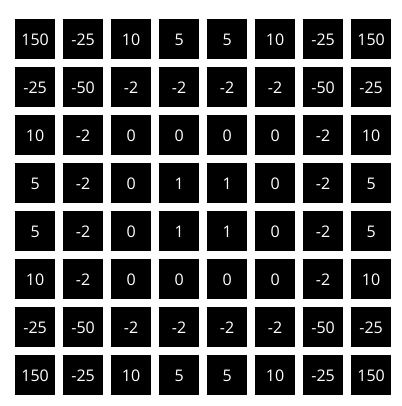
\includegraphics[scale=0.65]{./presentation/matrice-poids.png}
        \caption{Tableau de poids des cellules du plateau du Reversi}
        \label{fig:tab-prio}
    \end{figure}
\end{frame}

\subsection{Algorithme MinMax}
\begin{frame}
    Utilisation de l'algorithme MinMax :
    \begin{itemize}
        \item L'ordinateur cherche à maximiser son score : noeuds max (en rouge);
        \item Le joueur cherche à minimiser le score de l'ordinateur : noeuds min (en gris).
    \end{itemize}
    \begin{figure}
    \centering
    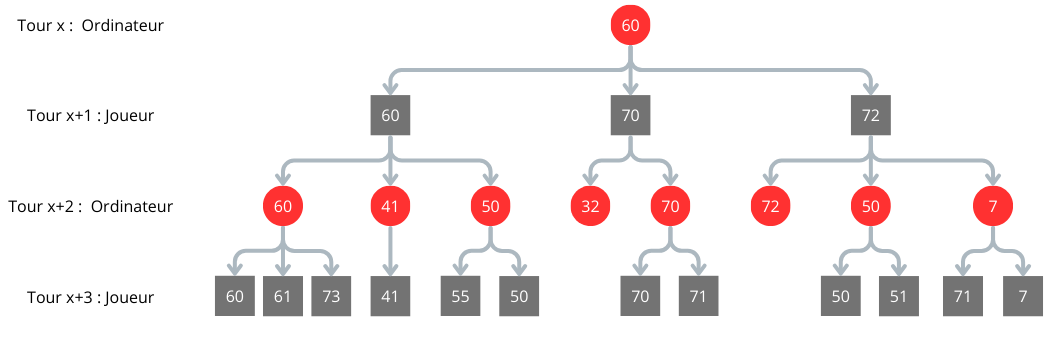
\includegraphics[scale=0.4]{./presentation/min-max.png}
    \caption{Illustration d’un arbre de jeu pour l’ordinateur}
    \label{fig:min-max}
    \end{figure}
\end{frame}

\section{Amélioration du parcours de l'arbre}
\begin{frame}{Amélioration du parcours de l'arbre}
    Utilisation de l'algorithme d’élagage AlphaBeta :
    \begin{itemize}
        \item Ordinateur : si le poids(noeud) $\geq$ poids(tonton) : élagage bêta
        \item Joueur : si le poids(noeud) $\leq$ poids(tonton) : élagage alpha
    \end{itemize}
    \begin{figure}
    \centering
    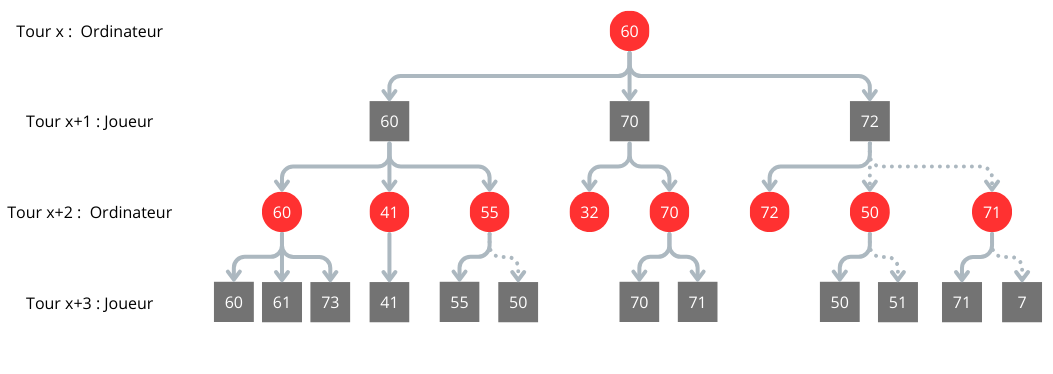
\includegraphics[scale=0.4]{./presentation/alpha-beta.png}
    \caption{Illustration d’un arbre de jeu pour l’ordinateur après élagage}
    \label{fig:alpha-beta}
    \end{figure}
\end{frame}

\section{Optimisation de la gestion de la mémoire}
\begin{frame}{Optimisation de la gestion de la mémoire}

\begin{itemize}
    \item Revu de la structure de l'arbre :
    \begin{itemize}
        \item suppression du plateau pour libérer de l'espace;
        \item ajout de coup;
        \item ajout des bornes pour retourner les pions. 
    \end{itemize}
    \item Utilisation direct du plateau de jeu que l'on modifiera en jouant puis annulant les coups lors de la création de l'arbre :
    \begin{itemize}
        \item problème : difficultés a revenir a l'état d'origine après calcul des fils;
        \item solution : copie du plateau lors de la descente puis suppression lors de la remontée.
    \end{itemize}
\end{itemize}
    
\end{frame}

\section{Pour aller plus loin}
\begin{frame}{Pour aller plus loin}
    Ce que nous avons mis en place :
    \begin{itemize}
        \item l'odinateur essaye maintenant de limiter les coups adverse;
        \item les "combos" de pions plus importants sont valorisés en fin de partie;
        \item ordinateur contre ordinateur
    \end{itemize}

    Idées supplémentaires :
    \begin{itemize}
        \item ajuster la matrice de poids au fil de la partie.
    \end{itemize}
\end{frame}

\end{document}
